\documentclass{school-22.211-notes}
\date{February 27, 2012}

\begin{document}
\maketitle

%%%%%%%%%%%%%%%%%%%%%%%%%%%%%%%%%%%%%%%%%%%%%%%%%%%%%%%%%%%
\lecture{Physical Concepts Related To Resonance Models}
\topic{Summary: Reuss Ch 8 Resonance Methods}
\begin{enumerate}
\item Self-shielding (Intro): 
  \begin{enumerate}
  \item Resonance capture xs can be tens of thousands of barns, but self-shielding makes sure that resonant capture of neutrons remains limited. That is, even with an $\infty$ xs, the probability of falling in the trap is limited, or even small, if the trap is narrow. 
  \item Explaination: `kangaroo leaps' tell us that the resonant capture probability is just trap width in lethargy divided by the average lethargy gain acquired by a neutron. 
  \item \textit{Compared to slowing down by moderator, the resonance of capture by the fuel are always narrow}.
  \item Technical term: absorption rate of neutrons remain approximately constant; that is, $\Phi \sim \frac{1}{\Sigma_a}$. 
  \item Self-shielding occurs at resonant energies, and in regions containing resonant material. 
  \end{enumerate}
\item Derivation of $\Phi(u)  = \frac{C}{\Sigma_t(u)}$ (8.1.1): starting from slowing down equation,
  \eqn{    \rho(u) + \overbrace{S(u)}^{\to 0} = \Sigma_t (u) \Phi(u) } 
  Before resonance the flux is asymptotic without absorption:
  \eqn{ \Phi(u) \approx \frac{q(u)}{\xi \Sigma_s (u)} = \frac{q}{\xi \Sigma_s} = \mbox{Constant} }
  Then the arrival density in the resonance is constant as well:
  \eqn{ \rho(u) = \Sigma_s (u) \Phi (u) = \frac{q}{\xi} = C}
  Plug back into the slowing down equation, we get the flux in the resonance:
  \eqn{ \Phi(u) \approx \frac{q}{\xi \Sigma_t (u)} = \frac{C}{\Sigma_t(u)} }
\item Derivation of resonance escape probability formula (8.1.2): 
  \eqn{P_{abs}  = \Sigma_a (u) \Phi (u) \du = \frac{\Sigma_a(u) \du}{\xi \Sigma_t (u)} }
  \eqn{p = 1 - P_{abs} = 1 - \Sigma_a(u) \Phi(u) \du = \exp \left( - \frac{\Sigma_a \du}{\xi \Sigma_t}  \right) }
(compare with the derivation we had in class)
\item Fine structure/self-shielding factor $\phi$ captures the detailed resonances, whereas macroscopit flux $\Psi$ captures everything else (8.1.3).
\item Fine structure in homogeneous mixture (8.2):
  \begin{enumerate}
    \item We define dilution xs as: $\sigma_d = \frac{N_m}{N_r} \sigma_m$ (8.2.1). 
    \item Two models for transforming a heterogeneous situation into a homogeneous one: 
      at very wide resonance (low energy), and at very narrow resonance (high energy). 
  \end{enumerate}
\item Distinguish between the different cases: truely homogeneous mixture, two-isotope heterogeneous configuration, homogenized heterogeneous configuration, and arrays of rods. 
\item When a particle coming out of fuel is not necessarily interacting with moderator, that is in the case of tight rods, we use Dancoff factor C, which is the probability for a neutron leaving a fuel element of crossing the moderator without a collision. (8.3.4).
\item Derivation of resonance escape probability in a heterogeneous situation as in Table~\ref{p-formulas} (8.3.5).
\begin{table}
  \centering
  \begin{tabular}{|c|c|} \hline
    Homogeneous & $p = \exp \left[ - \frac{N_0 I_{\eff}}{(\xi \Sigma_s)_m}  \right]$ \\ \hline
    General & $p = \exp \left[ - \frac{V_C N_0 I_{\eff}}{\Sum_i (V \xi \Sigma_s)_i}  \right]$ \\  \hline
  \end{tabular}
  \caption{Resonance Escape Probability Formulas} \label{p-formulas}
\end{table}
\item Doppler Effect (8.4):
\begin{enumerate}
\item Origin: we can ignore thermal agitation in treating scattering, because scattering xs is fairly constant, so a small change in velocity (hence energy) does not change xs much. Whereas in absorption, near resonance peaks, a small change in velocity (hence energy) would cause a huge difference in absorption xs, hence taking into account thermal agitation of the fuel material would make a difference. 
\item Characteristics 1: as temperatures increase, the resonance widens, and the peak is lowered, but with a constant resonance integral (area under the curve). 
\item Characteristics 2: although integral is constant, self-shielding says that \textit{the widening of the resonances has a much greater effect than the lowering of the peaks}. That is, Doppler effect as a whole leads to an increase in resonant capture by U238. 
\item $\RI_{\eff}$ for capture by U238 varies approximately linearly with the square root of dilution xs; it also varies linearly with the square root of absolute temperature. 
\end{enumerate}

\end{enumerate}



\topic{Resonance Integrals vs. Group Cross Section}
We introduce \hi{(Infinite) Resonance Integrals} as flux weighted (that is, weighted with 1/E spectrum $\phi(E) \sim \frac{1}{E}$) microscopic cross section: 
\begin{align}
\RI &=  - \int_{u1}^{u2} \sigma(u) \du \\
u &= \ln \left( \frac{E_0}{E} \right) = \ln(E_0) - \ln E \\
\du &= - \frac{1}{E} \dE \\ 
\RI &=  \int \sigma (E) \frac{1}{E} \dE 
\end{align}
Notice, 
\begin{itemize}
\item RI is defined directly from cross section data; no flux calculation is required because 1/E spectrum is assumed; 
\item RI depends on the normalization of the 1/E flux spectrum; it is also implicitly assumed that flux equals 1 when $E = 1$ through normalization;
\item RI is independent of energy bounds for isolated resonances;
\item RI is independent of temperature. This is because if the energy bound is larger enough, then as temperature increases, the spectrum would broaden, but because the area under the curve remains the same, assume the cross section is constant, then RI is essentially integrating the spectrum, which would not change upon temperature change;
\item RI is useful for inter-comparing libraries or cross section models. It is a classic way to evaluate new resonance data typically from 0.5 eV to 10 keV. We use RI to check our resonance data, in particularly the three big resonances at 6.67, 21, 26 eV. Numerical test of the SLBW RIs shows that the RI comes out to be within 1\% of ENDF/B-VII Reich-Moore data (Lec 6, slide 17, with 0.01 eV as spacing in histogram). 
\end{itemize}

\hi{Group cross section} is a similar but much more useful quantity. From its definition, we see $\sigma_g$ does not depend on the flux normalization: 
\begin{align}
\sigma_g &= \frac{\int_{E_1}^{E_2} \sigma(E) \phi(E) \dE }{\int_{E_1}^{E_2} \phi(E) \dE} 
\end{align}
If we make assumptions on the flux spectrum, then we can relate $\sigma_g$ to $\RI_{\eff}$,
\begin{align}
\phi(E) &\sim \frac{1}{E} \\
\sigma_g &= \frac{\int_{E_1}^{E_2} \sigma(E) \frac{1}{E} \dE }{\int_{E_1}^{E_2} \frac{1}{E} \dE} 
= \frac{\RI_{\eff}}{\ln(E_2) - \ln(E_1)}  
= \frac{\RI_{\eff}}{\ln(E_2/E_1)} \\
\Aboxed{\RI_{\eff} &= \sigma_g \ln(E_2/E_1) } \label{RIeff}
\end{align}
Notice\footnote{Review here for exam}:
\begin{itemize}
\item Group cross section by definition depends on both cross section and flux spectrum. 
\item Group cross section depends on the flux, but not on the normalization of flux (that is, only the shape matters, not the magnitude);
\item Group cross section depend explicitly on energy bounds (widths) of the groups; 
\item Effective RI can be computed from group cross sections and group energy bounds as in Eq.~\ref{RIeff}; As spectrum approaches 1/E, the effective RI computed from group cross sections will approach infinite RI. 
\end{itemize}

\topic{Temperature Effects On Cross Section (Doppler Broadening)}
\hi{Doppler Broadening} means, as the temperature increases, the width of the spectrum decreases, though the area under the curve stays the same. There are two possibilities: 
\begin{enumerate}
\item Infinite RI (infinite dilution factor) is independent of temperature becase the area under the psi chi curves are constant. 
\item Effective RI (finite concentration of \ce{^{238} U}) is dependent of temperature because of the self-shielding effect: as temperature increases, $\RI_{\eff}$ would increase. Also, as U/H increases, the fraction change of $\RI_{\eff}$ would increase as well as illustrated in Figure~\ref{Doppler}. That is, \textit{The higher the concentration of U238, the larger the Doppler temperature effects become.}
\end{enumerate}

In general, doppler broadening is the broadening of spectral lines due to the Doppler effect caused by a distribution of velocities of atoms or molecules. There are a couple of different kinds of Doppler broadening, including the thermal Doppler broadening due to the thermal motion of the particles; also, there are broadening depends on the frequency of the spectral line, the mass of the emitting particles, and the temperatures. 

Reference 1: Reuss Section 8.4. 

Reference 2: Handbook of Nuclear Engineering Chapter 4 Section 3. 

\begin{figure}
  \centering
  \subfloat[U/H=0.01]{\label{UH0.01}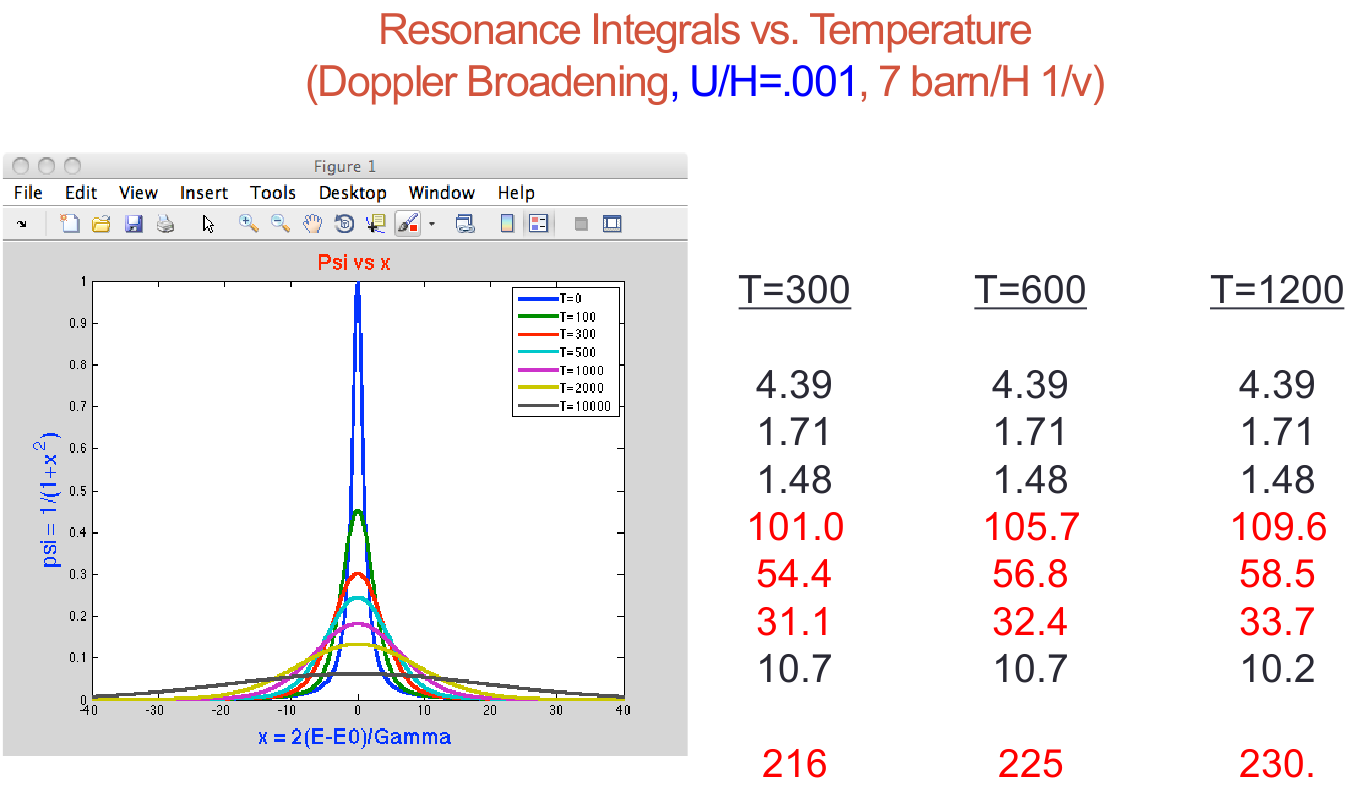
\includegraphics[width=0.5\textwidth]{images/Doppler-RI-1.png}}
  \subfloat[U/H=0.1]{\label{UH0.1}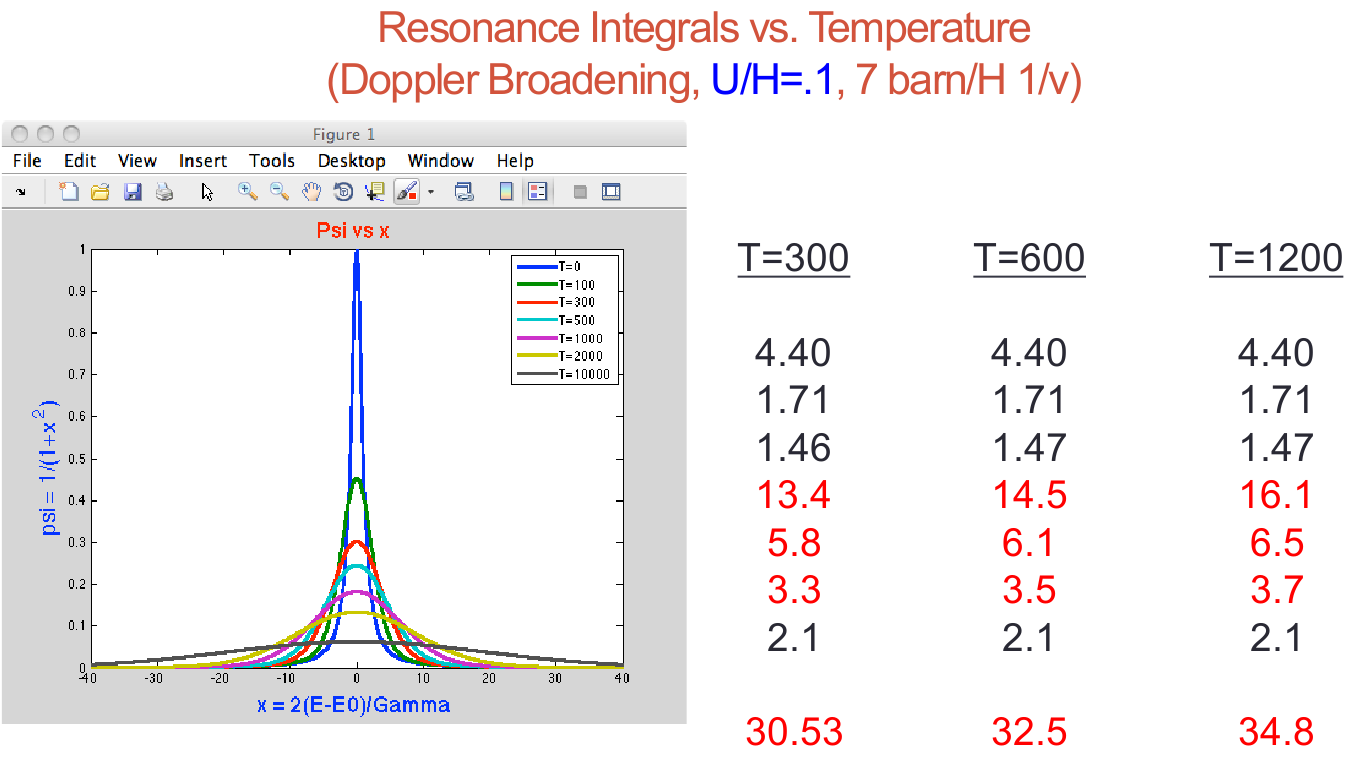
\includegraphics[width=0.5\textwidth]{images/Doppler-RI-2.png}}  
  \caption{Impact of Temperature On Effective RI/Resonance Absorption, Doppler Broadening} \label{Doppler}
\end{figure}


\topic{Energy Self-Shielding Effects On Spectrum}
As we increase the U/H ratio, the RI decreases in the three big resonance regions, and we see big dips on the spectrum plot. When U/H = 1.0, the spectrum is distorted. There are so much U238 in the fuel, that there is no flux in the fuel anymore. As we increase the number of uranium atoms by a factor of 10, the number of absorption per atom is decreased by a factor of 3. That is, the total aborption still increases, but the absorption per atom decreases. Figure~\ref{self-shielding} illustrates that RI are very dependent on the density of resonant materials. 
\begin{figure}
  \centering
  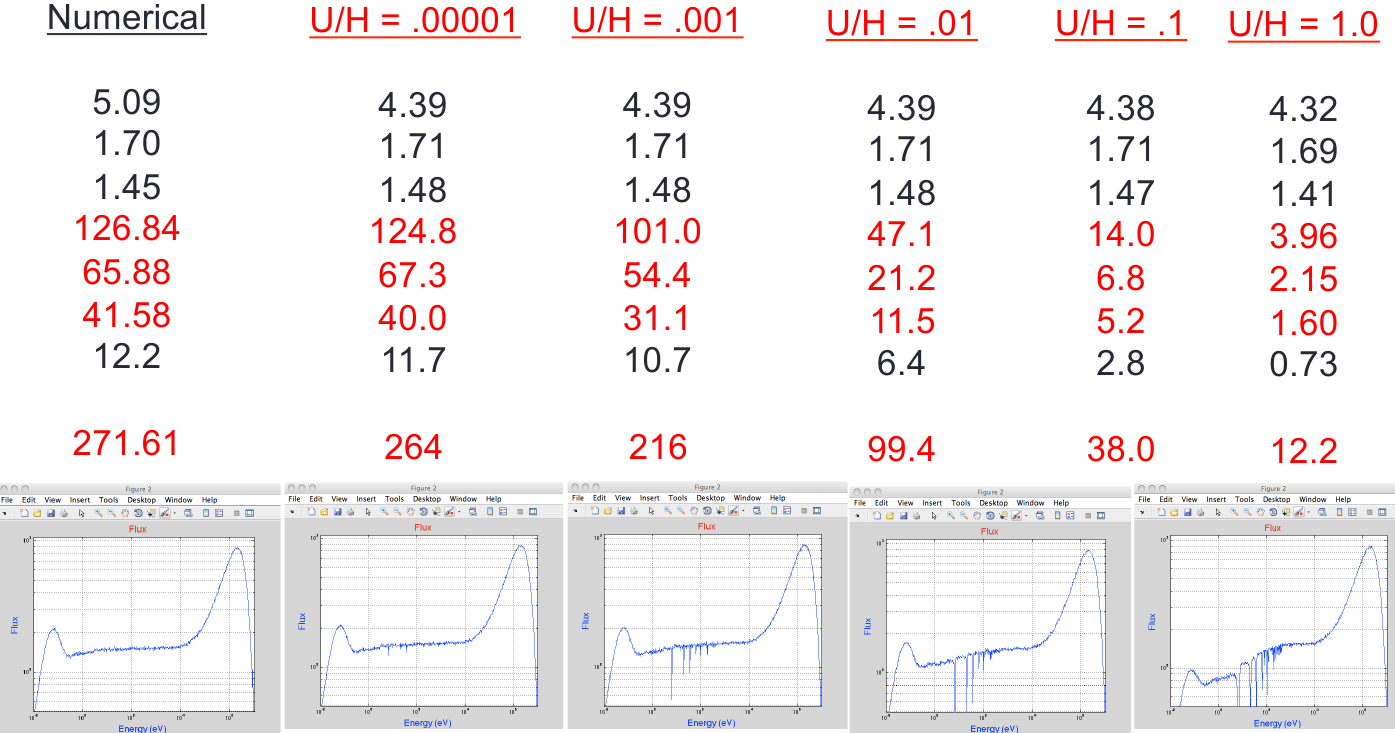
\includegraphics[width=4in]{images/self-shielding.png}
  \caption{Impact of Energy Self-Shielding On RI} \label{self-shielding}
\end{figure}


\topic{Spectral Hardening Shifts Resonant Absorption Rates}
\textit{As more absorber (uranium in this case) is added, the higher energy ranges become more important (more absorption happens in the higher energies), and the peak of the thermal spectrum shifts to the right.} Figure~\ref{spectral-hardening} also illustrates that self-shielding reduces the large resonance absorption fractions. 1/v absorption of U238 become more significant. 
\begin{figure}
  \centering
  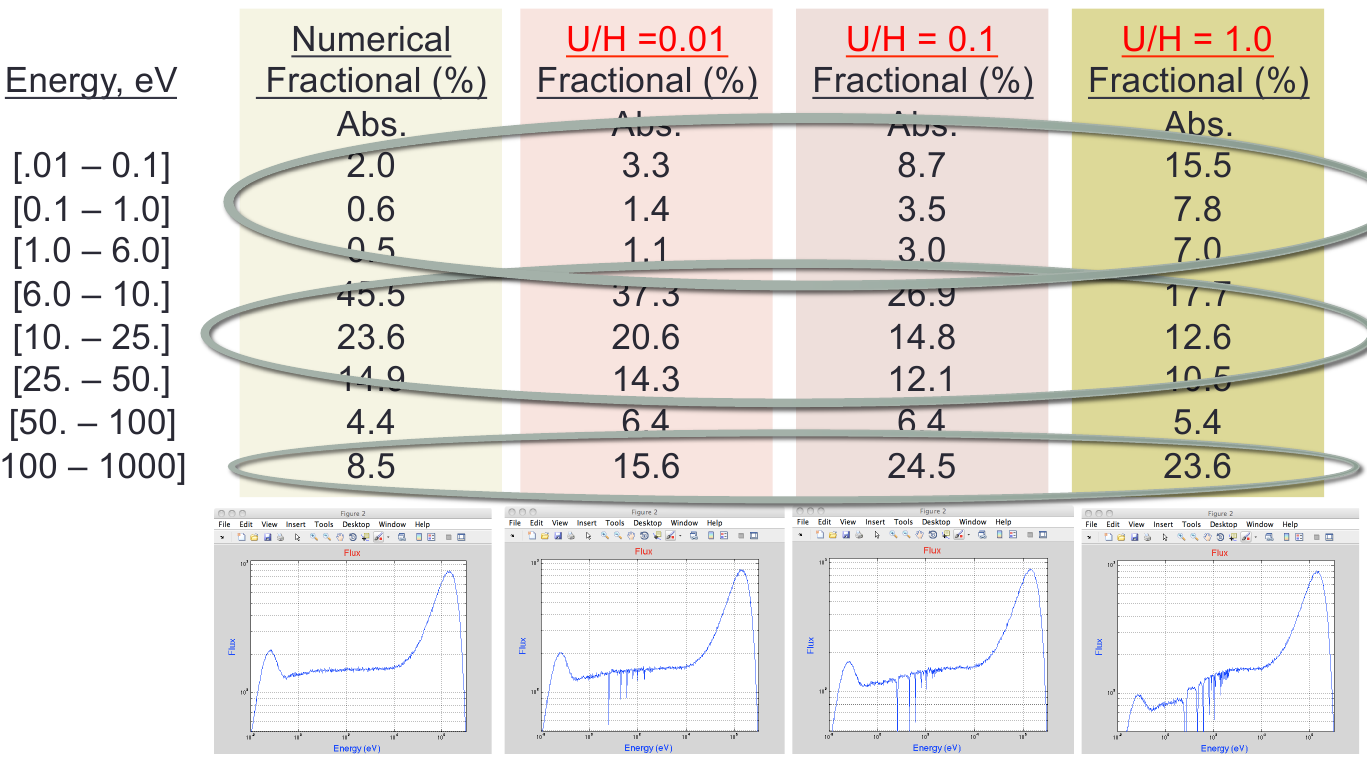
\includegraphics[width=4in]{images/spectral-hardening.png}
  \caption{Impact of Spectral Hardening On RI} \label{spectral-hardening}
\end{figure}


\end{document}
